\documentclass[12pt,a4paper]{article}
\usepackage[utf8]{inputenc}
\usepackage[T1]{fontenc}
\usepackage{amsmath}
\usepackage{amsfonts}
\usepackage{amssymb}
\usepackage{graphicx}
\usepackage{hyperref}
\usepackage[polish]{babel}
\usepackage{algorithm}
\usepackage{algpseudocode}
\usepackage{booktabs}
\usepackage{float}

% Fix for Polish algorithm name
\makeatletter
\def\ALG@name{Algorytm}
\makeatother

% Allow algorithms to float but keep them in the same section
\floatplacement{algorithm}{tbp}

\title{Sprawozdanie z implementacji heurystyk przeszukiwania lokalnego dla zmodyfikowanego problemu komiwojażera}
\author{Filip Rosiak 151799  \and Eryk Stec 152948}
\date{\today}

\begin{document}

\maketitle

\begin{abstract}
W niniejszym sprawozdaniu przedstawiono implementację i analizę heurystyk przeszukiwania lokalnego dla zmodyfikowanego problemu komiwojażera. Problem polega na ułożeniu dwóch rozłącznych zamkniętych ścieżek, każda zawierająca około 50\% wierzchołków, minimalizując łączną długość obu ścieżek. Zaimplementowano i porównano metodę przeszukiwania w wersji stromej i zachłannej, startując z rozwiązań losowych i zachłannych, z dwoma rodzajami sąsiedztwa (międzytrasowa wymiana wierzchołków i wewnątrztrasowa wymiana krawędzi albo wierzchołków). Eksperymenty przeprowadzono na instancjach kroa200 i krob200 z biblioteki TSPLib.
\end{abstract}

\section{Opis problemu}
Rozważany problem jest modyfikacją klasycznego problemu komiwojażera. Dany jest zbiór wierzchołków i symetryczna macierz odległości pomiędzy dowolną parą wierzchołków. Zadanie polega na ułożeniu dwóch rozłącznych zamkniętych ścieżek (cykli), każda zawierająca 50\% wierzchołków (jeżeli liczba wierzchołków w instancji nie jest parzysta, to pierwsza ścieżka zawiera jeden wierzchołek więcej), minimalizując łączną długość obu ścieżek.

Do testów wykorzystano instancje \texttt{kroa200} i \texttt{krob200} z biblioteki TSPLib. Są to dwuwymiarowe instancje euklidesowe, gdzie dla każdego wierzchołka podane są dwie współrzędne, a odległość pomiędzy wierzchołkami jest odległością euklidesową zaokrąglaną do liczby całkowitej.

\section{Zaimplementowane algorytmy rozwiązań startowych}
W ramach zadania zaimplementowano następujące heurystyki konstrukcyjne:

\subsection{Algorytm najbliższego sąsiada}
Algorytm jest inspirowany metodą najbliższego sąsiada dla klasycznego problemu komiwojażera, dostosowany do rozważanego problemu z dwoma cyklami. Pseudokod algorytmu przedstawiono w Algorytmie~\ref{alg:initial_nearest_neighbor}.


\begin{algorithm}[H]
\caption{Algorytm najbliższego sąsiada dla zmodyfikowanego problemu komiwojażera}
\label{alg:initial_nearest_neighbor}
\begin{algorithmic}[1]
\State \textbf{Znajdź punkty startowe:}
\State Losowo wybierz wierzchołki $(s_1, s_2)$
\State Te wierzchołki będą punktami startowymi dla cykli $C_1$ i $C_2$

\State \textbf{Inicjalizuj cykle:}
\State $C_1 = [s_1]$
\State $C_2 = [s_2]$
\State Dostępne wierzchołki $A = \{0, 1, ..., n-1\} \setminus \{s_1, s_2\}$

\State \textbf{Naprzemiennie rozbudowuj cykle:}
\While{$A$ nie jest puste}
        \State Znajdź wierzchołek $v \in A$ najbliższy ostatniemu wierzchołkowi w $C_1$
        \State Dodaj $v$ do $C_1$
        \State Usuń $v$ z $A$
        
        \If{A nie jest puste}
            \State Znajdź wierzchołek $v \in A$ najbliższy ostatniemu wierzchołkowi w $C_2$
            \State Dodaj $v$ do $C_2$
            \State Usuń $v$ z $A$
        \EndIf
\EndWhile

\State \Return $(C_1, C_2)$
\end{algorithmic}
\end{algorithm}

\newpage
\subsection{Rozwiązanie losowe}
Algorytm generuje cykle z losowo wybranymi wierzchołkami~\ref{alg:initial_random}.

\begin{algorithm}[H]
\caption{Algorytm inicjalizacji losowej dla zmodyfikowanego problemu komiwojażera}
\label{alg:initial_random}
\begin{algorithmic}[1]
\State \textbf{Inicjalizuj wierzchołki:}
\State $A = \{0, 1, ..., n-1\}$

\State \textbf{Potasuj wierzchołki:}
\State Potasuj elementy zbioru $A$

\State \textbf{Podziel wierzchołki na dwa cykle:}
\State $C_1 = A[0 : \lfloor n / 2 \rfloor]$
\State $C_2 = A[\lfloor n / 2 \rfloor : n]$

\State \Return $(C_1, C_2)$
\end{algorithmic}
\end{algorithm}

\newpage

\section{Zaimplementowane algorytmy generowania sąsiedztwa}
W ramach zadania zaimplementowano następujące algorytmy:

\subsection{Wymiana wierzchołków}
Algorytm generuje sąsiedztwo zawierające wszystkie możliwe wymiany międzytrasowe wierzchołków oraz wymiany wewnątrztrasowe wierzchołków~\ref{alg:neighborhood_vertices}.


\begin{algorithm}[H]
\caption{Generowanie ruchów - Wymiana wierzchołków}
\label{alg:neighborhood_vertices}
\begin{algorithmic}[1]
\State \textbf{Inicjalizuj sąsiedztwo}
\State $S = []$
\State \textbf{Generowanie ruchów między cyklami:}
\For{$i = 0$ to $|C_1| - 1$}
    \For{$j = 0$ to $|C_2| - 1$}
        \State Oblicz koszt wymiany wierzchołków $i$ i $j$ pomiędzy cyklami $C_1$ i $C_2$:
        \State Oblicz nowe koszty cykli
        \State Dodaj ruch do sąsiedztwa $S$
    \EndFor
\EndFor

\State \textbf{Generowanie ruchów w obrębie cykli:}
\For{$cycle\_num = 0$ to $1$}
    \For{$i = 0$ to $|C_{cycle\_num}| - 1$}
        \For{$j = i$ to $|C_{cycle\_num}| - 1$}
            \State Oblicz koszt wymiany wierzchołków w cyklu $C_{cycle\_num}$:
            \State Oblicz nowy koszt cyklu
            \State Dodaj ruch do sąsiedztwa $S$
        \EndFor
    \EndFor
\EndFor

\State \Return $S$
\end{algorithmic}
\end{algorithm}

\newpage
\subsection{Wymiana krawędzi}
Algorytm generuje sąsiedztwo zawierające wszystkie możliwe wymiany międzytrasowe wierzchołków oraz wymiany wewnątrztrasowe krawędzi~\ref{alg:neighborhood_edges}.

\begin{algorithm}[H]
\caption{Generowanie ruchów - Wymiana krawędzi}
\label{alg:neighborhood_edges}
\begin{algorithmic}[1]
\State \textbf{Inicjalizuj sąsiedztwo}
\State $S = []$
\State \textbf{Generowanie ruchów między cyklami:}
\For{$i = 0$ to $|C_1| - 1$}
    \For{$j = 0$ to $|C_2| - 1$}
        \State Oblicz koszt wymiany wierzchołków $i$ i $j$ pomiędzy cyklami $C_1$ i $C_2$:
        \State Oblicz nowe koszty cykli
        \State Dodaj ruch do sąsiedztwa $S$
    \EndFor
\EndFor

\State \textbf{Generowanie ruchów w obrębie cykli:}
\For{$cycle\_num = 0$ to $1$}
    \For{$i = 0$ to $|C_{cycle\_num}| - 1$}
        \For{$j = i$ to $|C_{cycle\_num}| - 1$}
            \State Oblicz koszt wymiany krawędzi w cyklu $C_{cycle\_num}$:
            \State Oblicz nowy koszt cyklu
            \State Dodaj ruch do sąsiedztwa $S$
        \EndFor
    \EndFor
\EndFor

\State \Return $S$
\end{algorithmic}
\end{algorithm}

\newpage

\section{Zaimplementowane algorytmy przeszukiwania lokalnego}
W ramach zadania zaimplementowano następujące przeszukiwania lokalnego:

\subsection{Algorytm Steepest Local Search}
Algorytm Steepest Local Search jest metodą przeszukiwania lokalnego, w której iteracyjnie generowane są możliwe ruchy w przestrzeni rozwiązań, a następnie wybierany jest najlepszy dostępny ruch prowadzący do najmniejszego kosztu. Algorytm kontynuuje proces, dopóki nie będzie już dostępny ruch prowadzący do lepszego rozwiązania. Pseudokod algorytmu przedstawiono w Algorytmie~\ref{alg:steepest_local_search}.

\begin{algorithm}[H]
\caption{Algorytm Steepest Local Search}
\label{alg:steepest_local_search}
\begin{algorithmic}[1]

\State $best\_cycles = [C_1.copy(), C_2.copy()]$
\State $best\_costs = \text{calculate\_total\_cost}(C_1, C_2, distance\_matrix)$

\While{True}
    \State \textbf{Generuj sąsiedztwo $S$}

    \State \textbf{Wybierz ruch o najmniejszym koszcie}

    \If{$best\_move\_costs \geq best\_costs$}
        \State \textbf{Zakończ:} Przerwij algorytm
    \EndIf

    \State \textbf{Aktualizacja kosztów i cykli:}
    \State $what\_swap, cycle\_num, i, j, new\_costs = best\_move$
    \State $best\_costs = best\_move\_costs$

    \If{$what\_swap = "vertices"$}
        \State \textbf{Wykonaj wymianę wierzchołków}
    \ElsIf{$what\_swap = "edges"$}
        \State \textbf{Wykonaj wymianę krawędzi}
    \Else
        \State \textbf{Wykonaj wymianę między cyklami}
    \EndIf
\EndWhile

\State \Return $best\_cycles, best\_costs$
\end{algorithmic}
\end{algorithm}

\newpage
\subsection{Algorytm Greedy Local Search}
Algorytm Greedy Local Search to metoda przeszukiwania lokalnego, w której  generowane są ruchy w przestrzeni rozwiązań, a następnie wybierany jest pierwszy ruch, który prowadzi do poprawy rozwiązania. Proces powtarza się, aż nie będzie już możliwe znalezienie lepszego rozwiązania w sąsiedztwie~\ref{alg:greedy_local_search}.

\begin{algorithm}[H]
\caption{Algorytm Greedy Local Search}
\label{alg:greedy_local_search}
\begin{algorithmic}[1]

\State $best\_cycles = [C_1.copy(), C_2.copy()]$
\State $best\_costs = \text{calculate\_total\_cost}(C_1, C_2, distance\_matrix)$

\While{True}
    \State \textbf{Generuj sąsiedztwo $S$}
    \State \textbf{Losowo przetasuj ruchy w sąsiedztwie} \Comment{random.shuffle()}

    \State \textbf{Próba poprawy rozwiązania:}
    \State $improved = False$
    \For{each move in $S$}
        \State $what\_swap, cycle\_num, i, j, new\_costs = move$
        \If{$new\_costs < best\_costs$}
            \State $best\_costs = new\_costs$
            \If{$what\_swap = "vertices"$}
                \State \textbf{Wykonaj wymianę wierzchołków}
            \ElsIf{$what\_swap = "edges"$}
                \State \textbf{Wykonaj wymianę krawędzi}
            \Else
                \State \textbf{Wykonaj wymianę między cyklami}
            \EndIf
            \State $improved = True$
            \State \textbf{Przerwij iterację w celu ponownego wygenerowania sąsiedztwa}
        \EndIf
    \EndFor

    \If{not $improved$}
        \State \textbf{Zakończ:} Przerwij algorytm
    \EndIf
\EndWhile

\State \Return $best\_cycles, best\_costs$
\end{algorithmic}
\end{algorithm}

\subsection{Random Walk}
Algorytm Random Walk to metoda przeszukiwania losowego, w której wykonywane są losowe ruchy w przestrzeni rozwiązań, a algorytm stara się znaleźć rozwiązanie o najniższym koszcie. W każdej iteracji wykonywany jest losowy ruch będący wymianą między cyklami lub wewnątrz cykli~\ref{alg:random_walk}.

\begin{algorithm}[H]
\caption{Algorytm Random Walk}
\label{alg:random_walk}
\begin{algorithmic}[1]

\State $start\_time = \text{time()}$
\State $best\_cycles = [C_1, C_2]$
\State $best\_costs = \text{calculate\_total\_cost}(C_1, C_2, distance\_matrix)$

\State $cycles = [C_1, C_2]$
\State $costs = best\_costs.copy()$

\While{$\textbf{time()} - start\_time < time\_limit$}
    \If{$\textbf{random()} < 0.5$}
        \State \textbf{Wykonaj wymianę między cyklami}


        \If{$costs < best\_costs$}
            \State $best\_cycles = cycles$
            \State $best\_costs = costs$
        \EndIf

    \Else
        \State \textbf{Wykonaj wymianę wewnątrz cykli}
        \State $cycle\_num = \text{randint}(0, 1)$
        \State $i, j = \text{random.sample}(range(|C_{cycle\_num}|), 2)$
        
        \If{$\text{random()} < 0.5$}
            \State \textbf{Wykonaj wymianę wierzchołków}
        \Else
            \State \textbf{Wykonaj wymianę krawędzi}
        \EndIf
        
        \State \textbf{Oblicz nowy koszt}

        \If{$costs < best\_costs$}
            \State $best\_cycles = cycles$
            \State $best\_costs = costs$
        \EndIf
    \EndIf
\EndWhile

\State \Return $best\_cycles, best\_costs$
\end{algorithmic}
\end{algorithm}

\newpage
\section{Wyniki eksperymentów}
Każdy algorytm został uruchomiony 100 razy na instancjach kroa200 i krob200 dla każdej kombinacji. Poniżej przedstawiono wyniki eksperymentów.

\begin{table}[H]
\centering
\caption{Wyniki eksperymentów dla instancji kroa200 i krob200}
\begin{tabular}{lcc}
\toprule
\textbf{Kombinacja} & \textbf{kroa200} & \textbf{krob200} \\
\midrule
Steepest\_vertices\_random & 73584 (63783 - 85227) & 71369 (57133 - 87696) \\
Steepest\_vertices\_greedy & 39135 (34563 - 45919) & 39302 (35937 - 42724) \\
Steepest\_edges\_random & 38619 (35788 - 41799) & 38784 (37002 - 40703) \\
Steepest\_edges\_greedy & 34214 (31474 - 37108) & 34752 (31941 - 37619) \\
Greedy\_vertices\_random & 66869 (56854 - 82352) & 65570 (55638 - 74526) \\
Greedy\_vertices\_greedy & 39280 (35094 - 45765) & 39370 (35862 - 42657) \\
Greedy\_edges\_random & 38778 (36125 - 41088) & 38747 (36277 - 40721) \\
Greedy\_edges\_greedy & 34979 (31636 - 37717) & 35432 (32078 - 38777) \\
Random\_walk & 281003 (271676 - 285587) & 276016 (270202 - 281053) \\
\bottomrule
\end{tabular}
\end{table}

\begin{table}[H]
\centering
\caption{Czasy eksperymentów dla instancji kroa200 i krob200}
\begin{tabular}{lcc}
\toprule
\textbf{Kombinacja} & \textbf{kroa200} & \textbf{krob200} \\
\midrule
Steepest\_vertices\_random & 4.90 (4.08 - 5.91) & 5.16 (4.08 - 6.35) \\
Steepest\_vertices\_greedy & 0.42 (0.20 - 0.63) & 0.36 (0.09 - 0.63) \\
Steepest\_edges\_random & 3.74 (3.32 - 4.16) & 3.89 (3.36 - 4.68) \\
Steepest\_edges\_greedy & 0.81 (0.58 - 1.21) & 0.75 (0.53 - 1.13) \\
Greedy\_vertices\_random & 17.62 (15.33 - 20.62) & 18.47 (15.47 - 23.48) \\
Greedy\_vertices\_greedy & 0.77 (0.25 - 1.59) & 0.59 (0.11 - 1.07) \\
Greedy\_edges\_random & 15.79 (14.07 - 18.07) & 16.56 (14.42 - 18.82) \\
Greedy\_edges\_greedy & 1.78 (1.16 - 2.79) & 1.57 (0.86 - 2.62) \\
Random\_walk & 17.62 (17.62 - 17.62) & 18.47 (18.47 - 18.47) \\
\bottomrule
\end{tabular}
\end{table}

\newpage

\section{Wizualizacje}
Poniżej przedstawiono wizualizacje najlepszych rozwiązań dla każdej kombinacji i instancji.

\subsection{Instancja kroA200}

\begin{figure}[H]
\centering
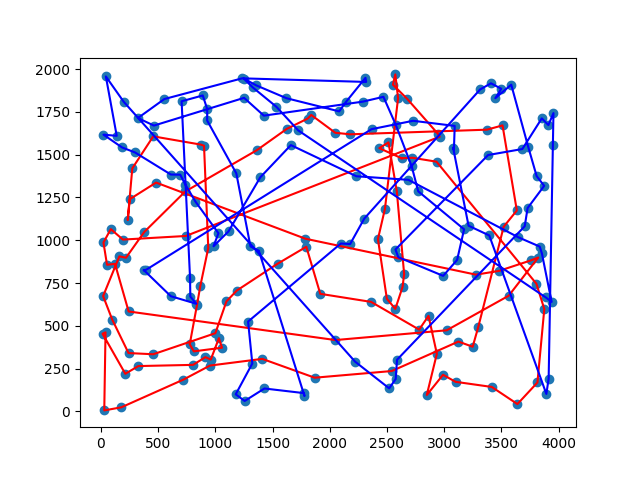
\includegraphics[width=0.8\textwidth]{figures/kroA_Steepest_V_random.png}
\caption{Rozwiązanie dla Steepest\_vertices\_random na instancji kroA200}
\end{figure}

\begin{figure}[H]
\centering
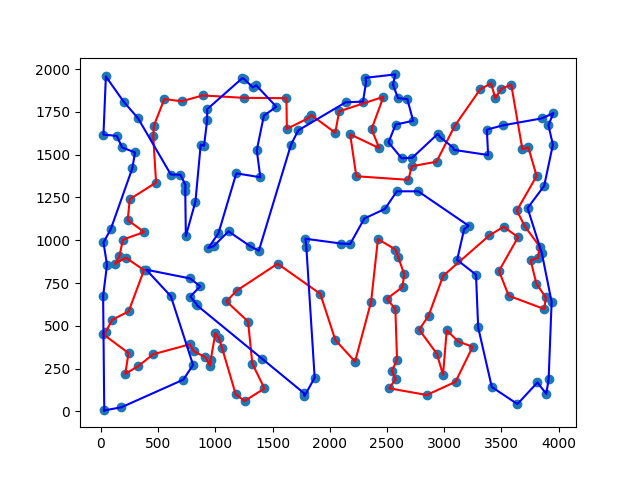
\includegraphics[width=0.8\textwidth]{figures/kroA_Steepest_E_random.png}
\caption{Rozwiązanie dla Steepest\_edge\_random na instancji kroA200}
\end{figure}

\begin{figure}[H]
\centering
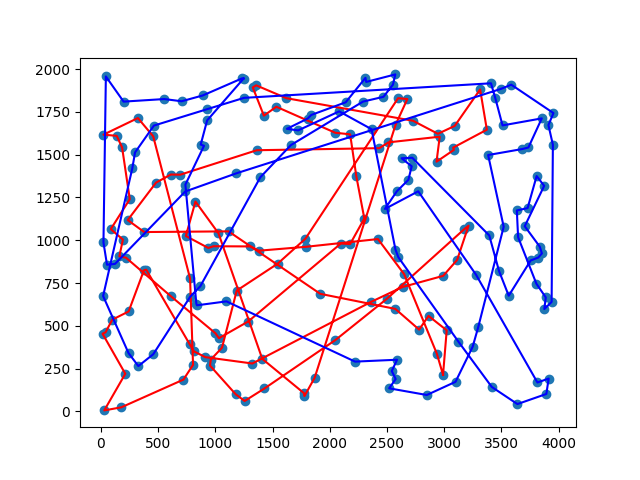
\includegraphics[width=0.8\textwidth]{figures/kroA_Greedy_V_random.png}
\caption{Rozwiązanie dla Greedy\_vertices\_random na instancji kroA200}
\end{figure}

\begin{figure}[H]
\centering
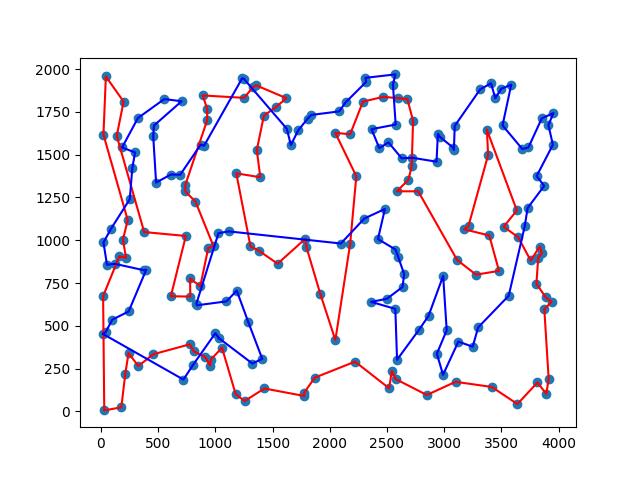
\includegraphics[width=0.8\textwidth]{figures/kroA_Greedy_E_random.png}
\caption{Rozwiązanie dla Greedy\_edge\_random na instancji kroA200}
\end{figure}

\begin{figure}[H]
\centering
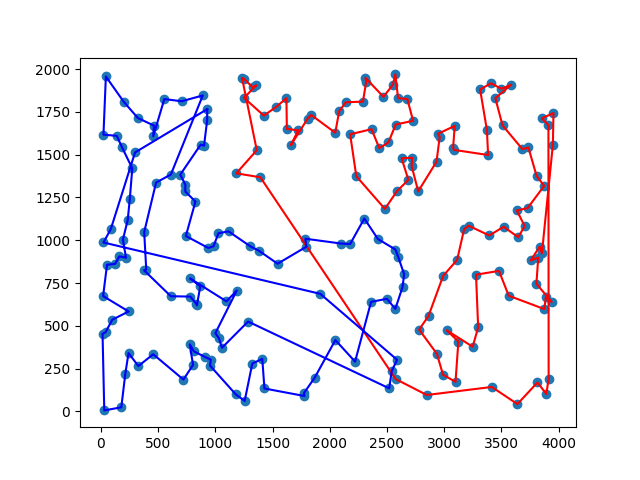
\includegraphics[width=0.8\textwidth]{figures/kroA_Steepest_V_greedy.png}
\caption{Rozwiązanie dla Steepest\_vertices\_greedy na instancji kroA200}
\end{figure}

\begin{figure}[H]
\centering
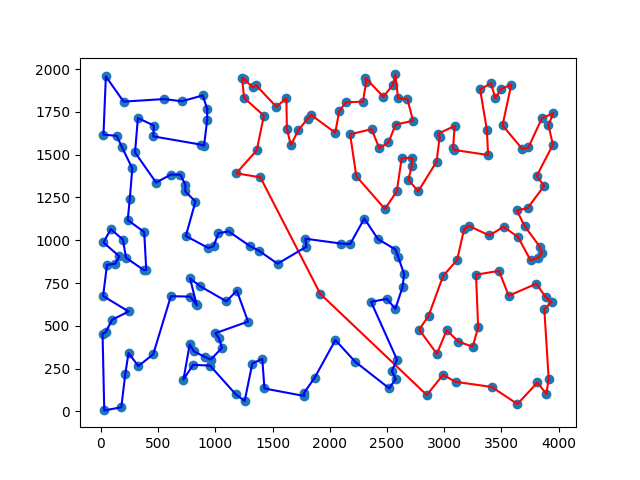
\includegraphics[width=0.8\textwidth]{figures/kroA_Steepest_E_greedy.png}
\caption{Rozwiązanie dla Steepest\_edge\_greedy na instancji kroA200}
\end{figure}

\begin{figure}[H]
\centering
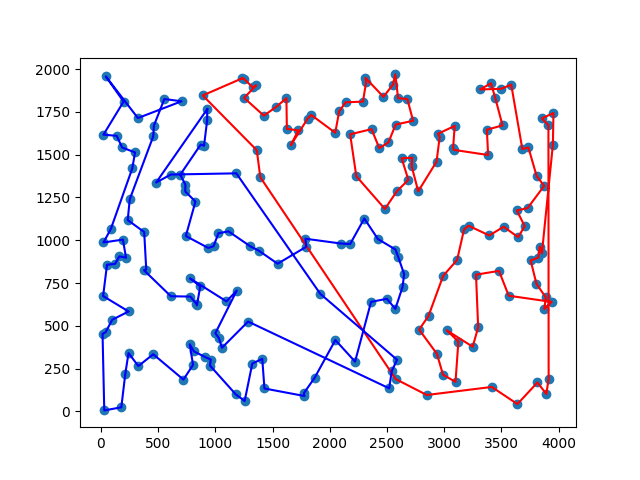
\includegraphics[width=0.8\textwidth]{figures/kroA_Greedy_V_greedy.png}
\caption{Rozwiązanie dla Greedy\_vertices\_greedy na instancji kroA200}
\end{figure}

\begin{figure}[H]
\centering
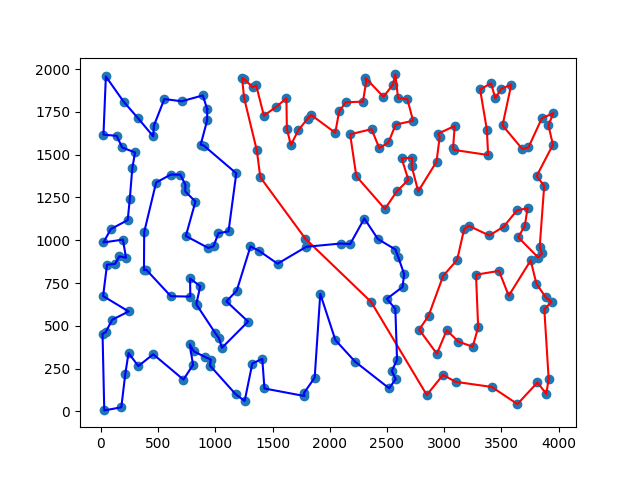
\includegraphics[width=0.8\textwidth]{figures/kroA_Greedy_E_greedy.png}
\caption{Rozwiązanie dla Greedy\_edge\_greedy na instancji kroA200}
\end{figure}

\begin{figure}[H]
\centering
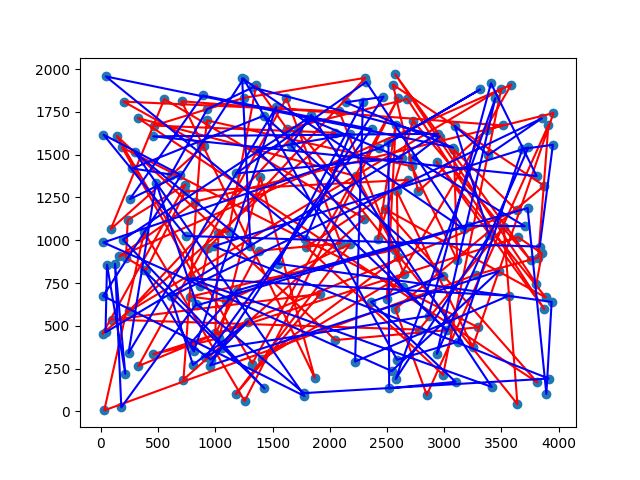
\includegraphics[width=0.8\textwidth]{figures/kroA_random_walk.png}
\caption{Rozwiązanie dla Random\_walk na instancji kroA200}
\end{figure}

\subsection{Instancja kroB200}

\begin{figure}[H]
\centering
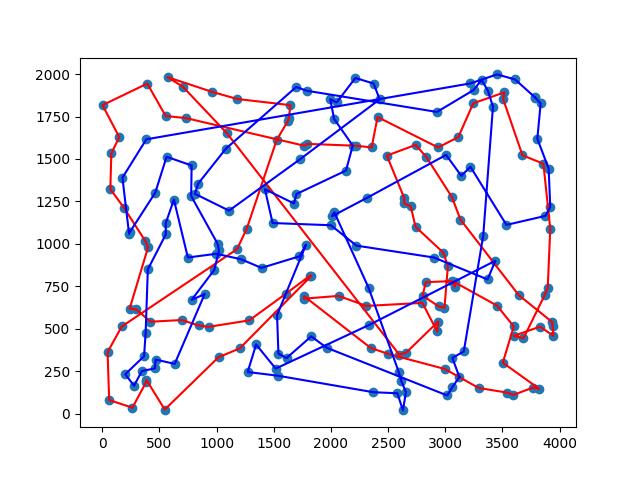
\includegraphics[width=0.8\textwidth]{figures/kroB_Steepest_V_random.png}
\caption{Rozwiązanie dla Steepest\_vertices\_random na instancji kroB200}
\end{figure}

\begin{figure}[H]
\centering
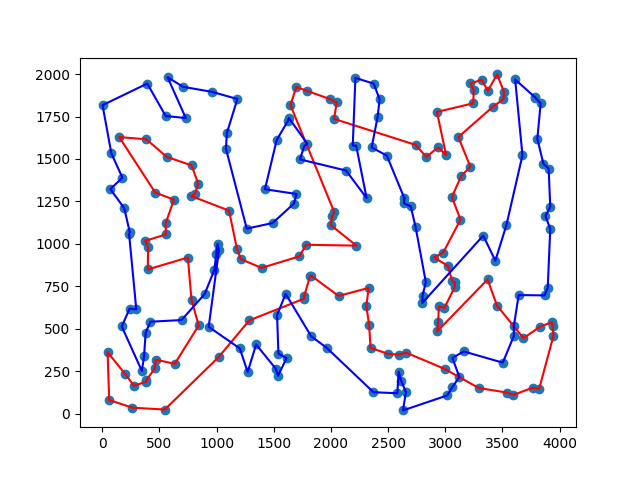
\includegraphics[width=0.8\textwidth]{figures/kroB_Steepest_E_random.png}
\caption{Rozwiązanie dla Steepest\_edge\_random na instancji kroB200}
\end{figure}

\begin{figure}[H]
\centering
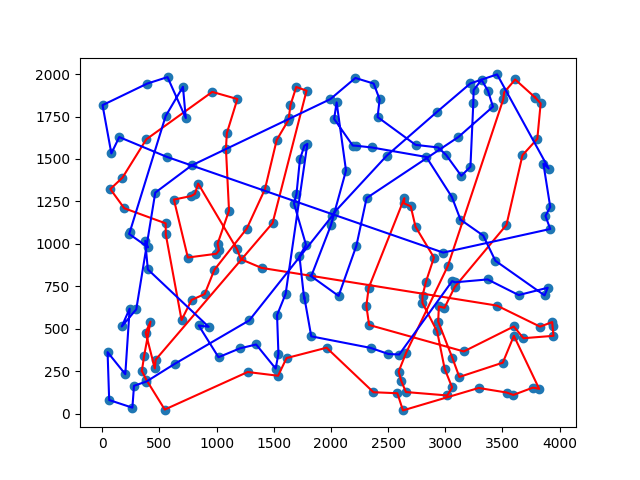
\includegraphics[width=0.8\textwidth]{figures/kroB_Greedy_V_random.png}
\caption{Rozwiązanie dla Greedy\_vertices\_random na instancji kroB200}
\end{figure}

\begin{figure}[H]
\centering
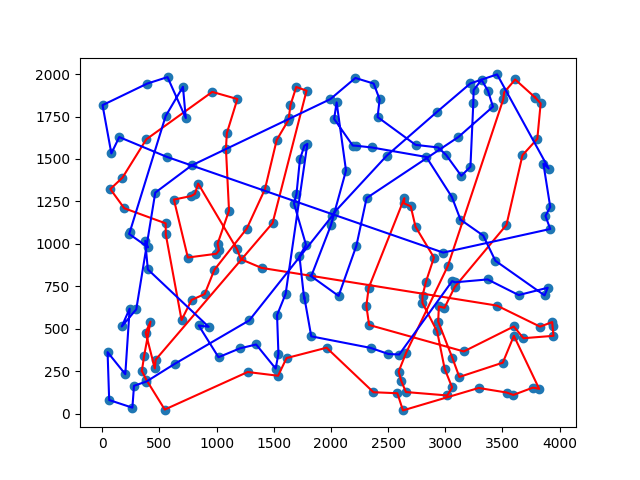
\includegraphics[width=0.8\textwidth]{figures/kroB_Greedy_V_random.png}
\caption{Rozwiązanie dla Greedy\_edge\_random na instancji kroB200}
\end{figure}

\begin{figure}[H]
\centering
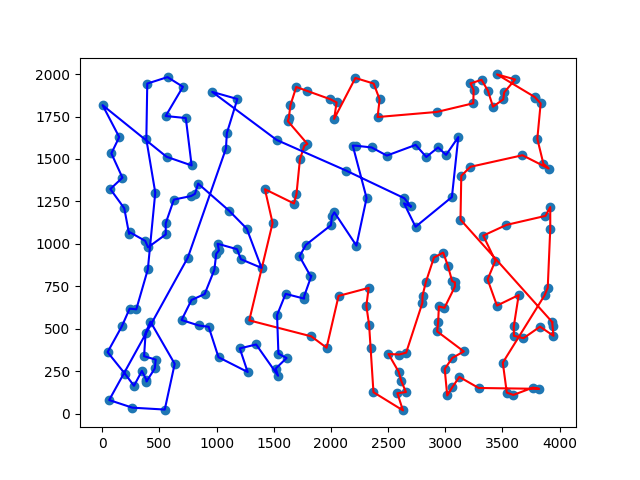
\includegraphics[width=0.8\textwidth]{figures/kroB_Steepest_V_greedy.png}
\caption{Rozwiązanie dla Steepest\_vertices\_greedy na instancji kroB200}
\end{figure}

\begin{figure}[H]
\centering
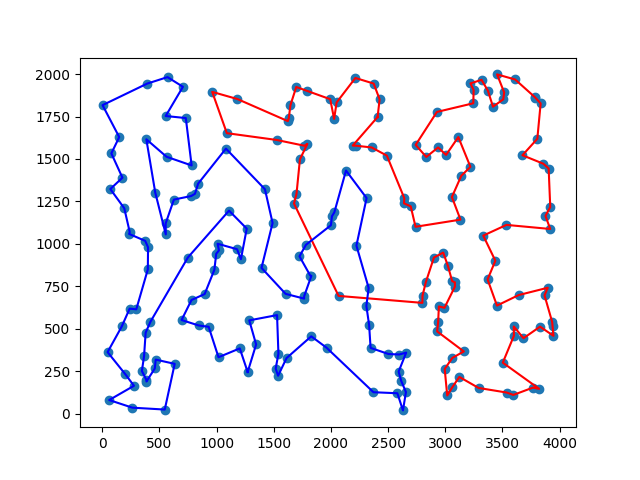
\includegraphics[width=0.8\textwidth]{figures/kroB_Steepest_E_greedy.png}
\caption{Rozwiązanie dla Steepest\_edge\_greedy na instancji kroB200}
\end{figure}

\begin{figure}[H]
\centering
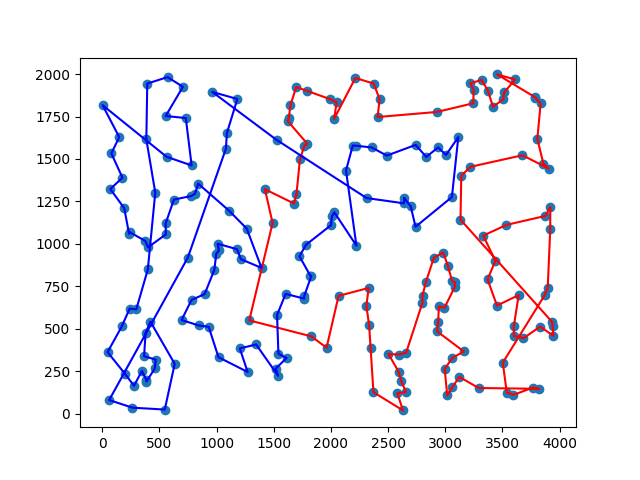
\includegraphics[width=0.8\textwidth]{figures/kroB_Greedy_V_greedy.png}
\caption{Rozwiązanie dla Greedy\_vertices\_greedy na instancji kroB200}
\end{figure}

\begin{figure}[H]
\centering
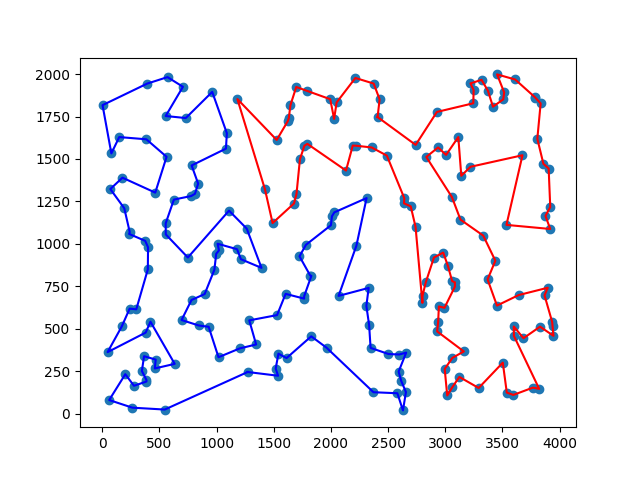
\includegraphics[width=0.8\textwidth]{figures/kroB_Greedy_E_greedy.png}
\caption{Rozwiązanie dla Greedy\_edge\_greedy na instancji kroB200}
\end{figure}

\begin{figure}[H]
\centering
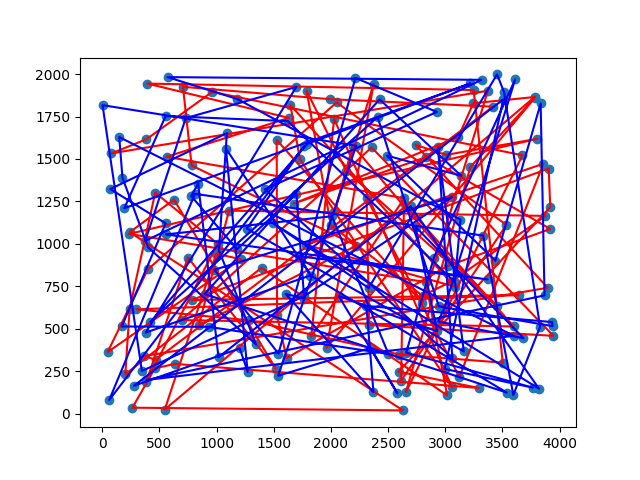
\includegraphics[width=0.8\textwidth]{figures/kroB_random_walk.png}
\caption{Rozwiązanie dla Random\_walk na instancji kroB200}
\end{figure}

\section{Wnioski}
Na podstawie przeprowadzonych eksperymentów można wyciągnąć następujące wnioski:

\begin{enumerate}

\item Najlepsze wyniki dla obu instancji osiągnęła kombinacja Steepest\_edges\_greedy czyli lokalne przeszukiwanie strome wykorzystujące zamianę krawędzi oraz posiadające rozwiązanie początkowe wykonane metodą zachłanną, uzyskując najniższe wartości funkcji celu (34214 dla kroa200 i 34752 dla krob200).

\item Metoda Steepest\_vertices\_greedy jest najszybsza (średni czas wykonania poniżej 0.5 sekundy), jednak jej wyniki są gorsze pod względem jakości rozwiązania (39135 dla kroa200 i 39302 dla krob200) w porównaniu do najlepszych metod opartych na krawędziach.

\item Metody oparte na strategii początkowym rozwiązaniu greedy oferują dobry kompromis między jakością rozwiązania a czasem wykonania, osiągając lepsze wyniki niż metody z losowym rozwiązaniem startowym przy znacznym skróceniu czasu obliczeń.

\item Metody wykorzystujące losowe rozwiązanie początkowe i zamianę wierzchołków są bardziej czasochłonne niż te bazujące na podejściu greedy, a ich wyniki są znacznie gorsze. Na przykład metoda Greedy\_vertices\_random uzyskała wynik 66869 dla kroa200 przy czasie 17.62 s.

\item Metoda losowego bładzenia jest najmniej efektywna zarówno pod względem jakości rozwiązania, jak i czasu wykonania. Uzyskała najgorsze wartości funkcji celu (281003 dla kroa200 i 276016 dla krob200) przy czasie działania równym czasowi najwolniejszego algorymu przeszukiwania.

\item Wyniki dla instancji kroa200 i krob200 są spójne, co sugeruje, że rozwiązania poszczególnych metod nie zależą od konkretnej instancji problemu.

\item W celu uzyskania najlepszej jakości rozwiązania powinno zastosować się metodę Steepest\_edges\_greedy lub Greedy\_edges\_greedy, natomiast jeśli priorytetem jest szybkość obliczeń,najlepszym wyborem wyborem będzie Steepest\_vertices\_greedy.

\item Najlepsze rezultaty można osiągnąć, łącząc podejście zachłanne do znalezienia rozwiązania początkowego z dalszą optymalizacją poprzez zamianę krawędzi. Strategia ta pozwala szybko uzyskać dobrą jakość rozwiązania, a następnie ulepszać je poprzez lokalne modyfikacje.

\end{enumerate}

\section{Kod źródłowy}
Pełny kod źródłowy implementacji wszystkich algorytmów jest dostępny w repozytorium GitHub:
\url{https://github.com/FilipRosiak1/IMO-2}

\end{document} 